\section{Punto de Vista de Tecnología}

El punto de vista de la tecnología contiene los elementos de tecnología de software y hardware que soportan la Capa de Aplicación, tales como dispositivos físicos, redes o software del sistema (por ejemplo, sistemas operativos, bases de datos y middleware). Un proceso tecnológico representa una secuencia de comportamientos tecnológicos que logran un resultado específico.

\subsection{Modelo de Tecnología}
\begin{figure}[h!]
	\centering
	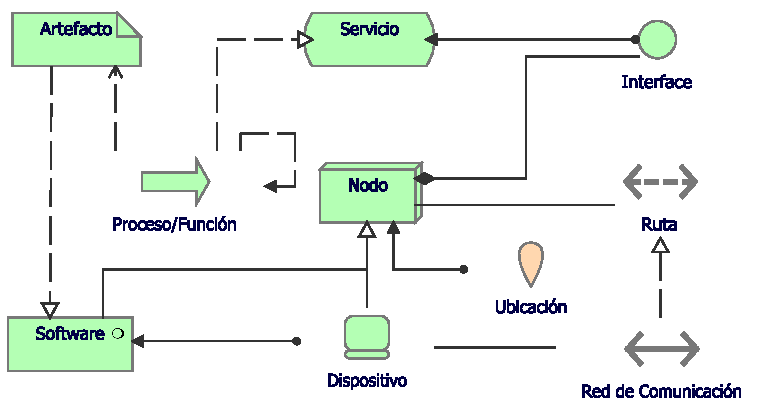
\includegraphics[width=.8\linewidth]{imgs/modelo/Tecnologia.pdf}
	\caption{Modelo de Tecnología}
\end{figure}

Por otra parte, un proceso tecnológico describe el comportamiento interno de un nodo; para el usuario de ese nodo, este proceso es invisible. Si su comportamiento es expuesto externamente, esto se hace a través de uno o más servicios de tecnología. Un proceso tecnológico se abstrae de la forma en que se implementa y sólo se especifica el comportamiento necesario. Así mismo, puede usar objetos tecnológicos como entrada y usarlos o transformarlos para producir otros objetos tecnológicos como salida. Un proceso tecnológico puede realizar servicios tecnológicos. Otros servicios tecnológicos pueden servir (ser utilizados por) un proceso tecnológico. Además, Un proceso tecnológico puede acceder a los objetos tecnológicos. Se puede asignar un nodo a un proceso tecnológico, lo que significa que este nodo realiza el proceso. El nombre de un proceso tecnológico debe identificar claramente una serie de comportamientos tecnológicos; por ejemplo, "Secuencia de arranque del sistema" o "Replicar la base de datos".

\newpage

\subsection{Caso  de Tecnología}
\begin{figure}[h!]
	\centering
	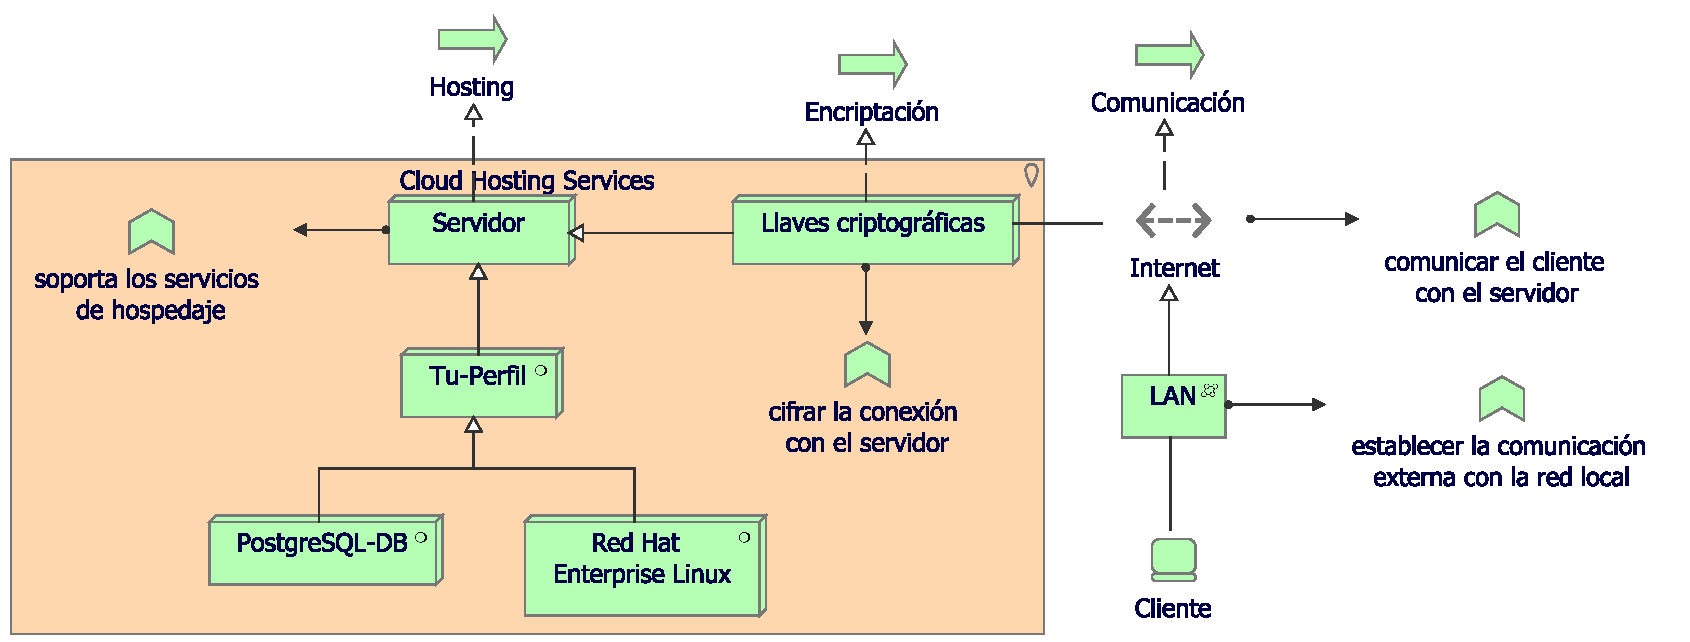
\includegraphics[width=1\linewidth]{imgs/puntos_vista/tecnologia/tecnologia}
	\caption{Caso de Tecnología}
\end{figure}

Para esta capa, algunos de los requerimientos funcionales del software Tu-Perfil, están soportados en una arquitectura serverless para el almacenamiento (hosting) de la aplicación; específicamente, a partir del servicio de plataforma en la nube, está compuesto de un AMI de Red Hat Enterprise 8 y un motor de base de datos PostgresSQL 13.  Asimismo, se dispone de un manejador de llaves encriptadas (KMS) para el cifrado de la conexión al servidor que contribuye con el proceso tecnológico de comunicación, a través de la red de comunicación global Internet.\\ 

Puesto que Internet conforma el elemento de ruta (o path) de nuestra capa tecnológica, se hace evidente que también hace referencia a la otra parte del proceso de comunicación encargado de la comunicación entre el cliente y el servidor de la aplicación. Luego, se dispone para el elemento de la capa, red de comunicación, una red de área local (LAN), la cual está encargada de establecer la comunicación externa con la intranet del dispositivo cliente de la arquitectura.